\documentclass[a4paper, 10pt, garamond]{book}
\usepackage{cours-preambule}

\begin{document}

\begin{adjustwidth}{-1cm}{-1cm}
  \pagestyle{empty}
  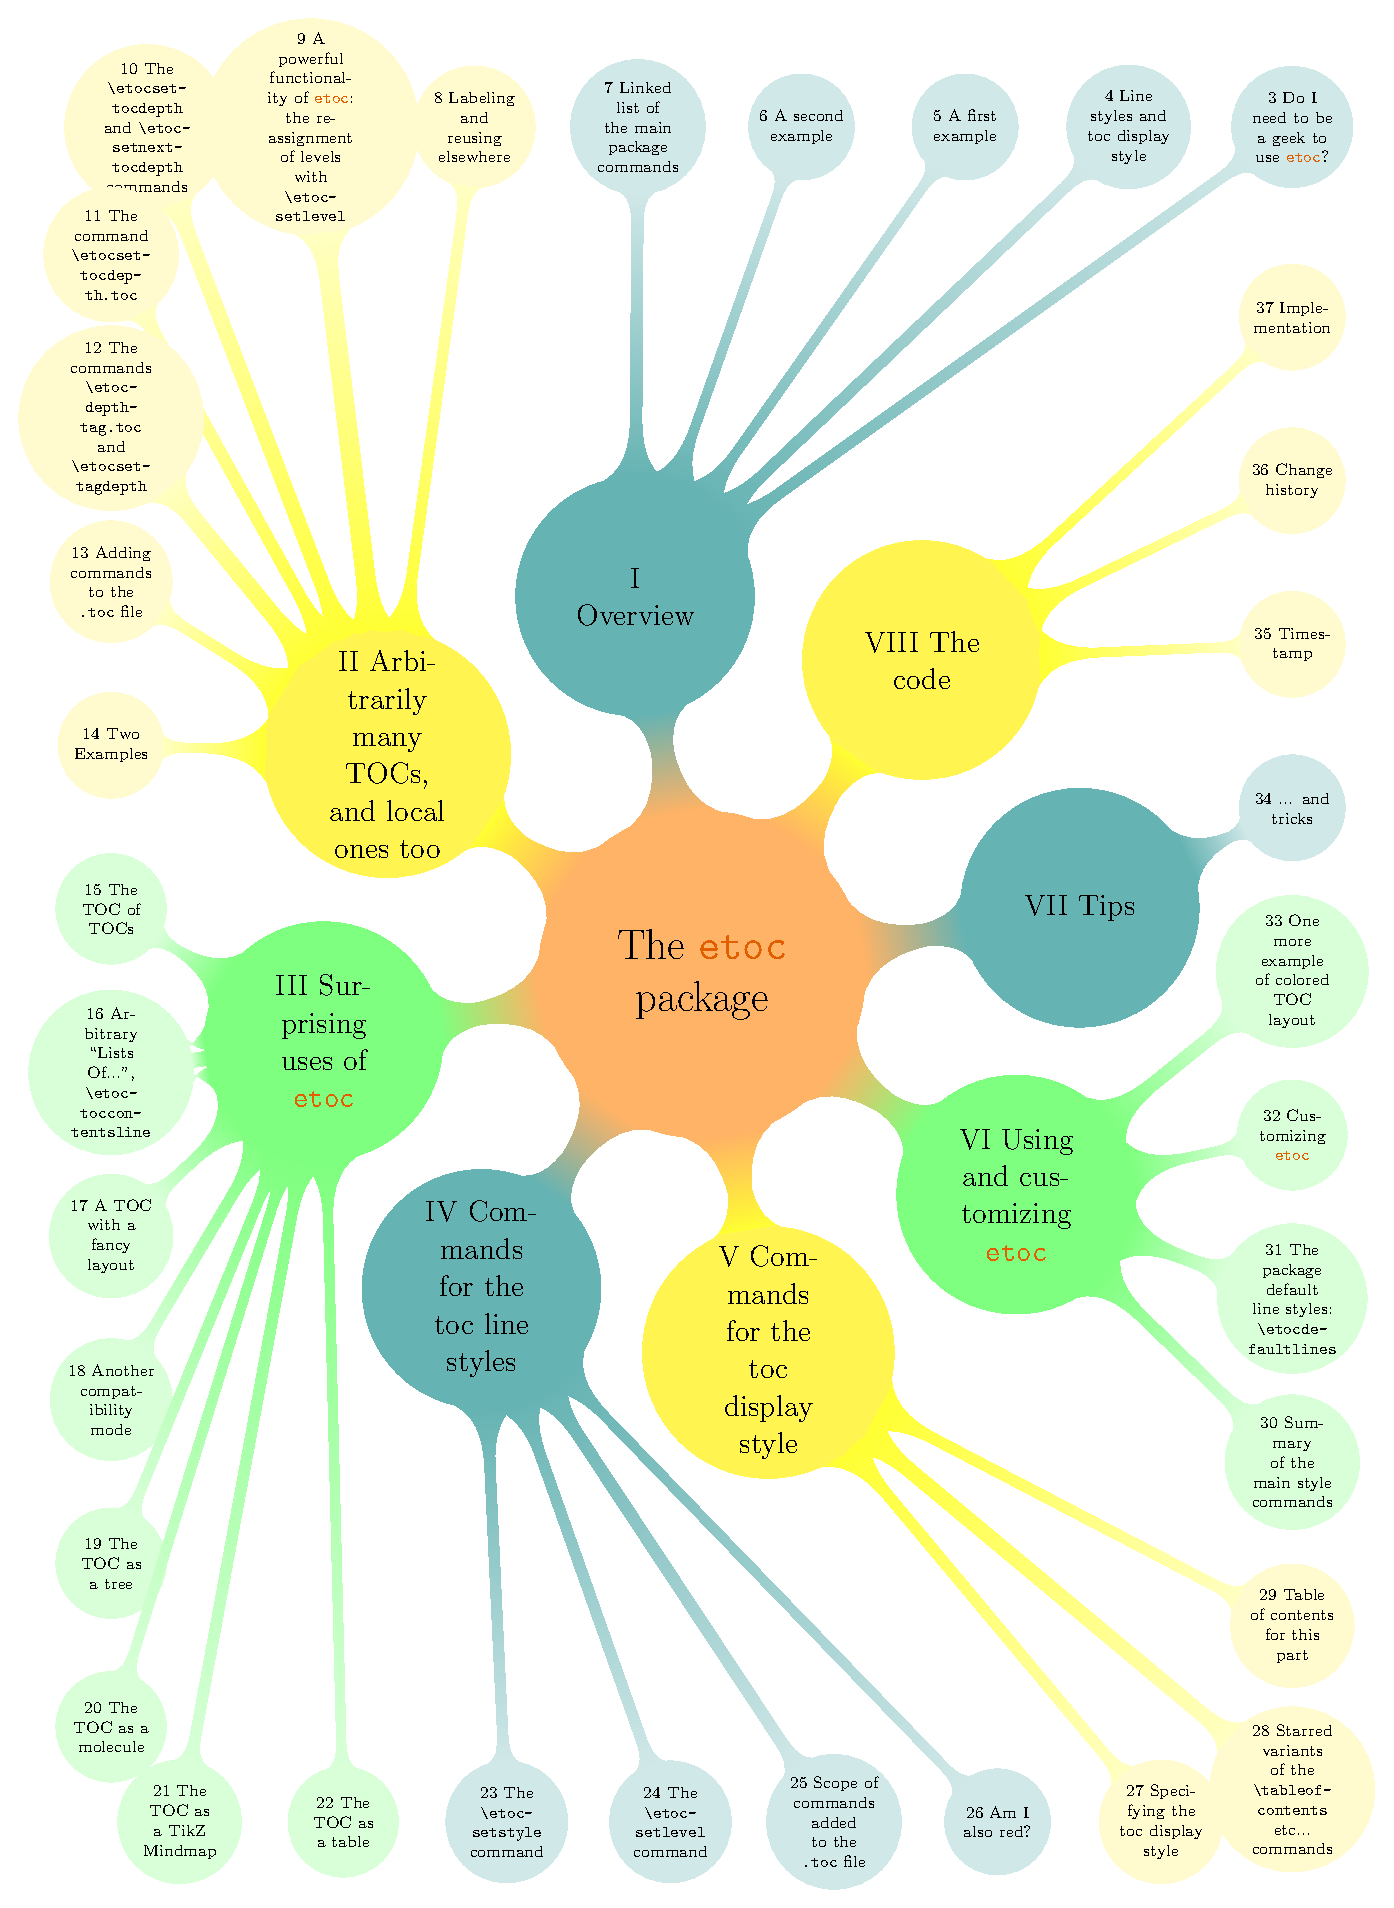
\includegraphics[width=\linewidth]{cover}
\end{adjustwidth}
\newpage

\tableofcontents
% \listoffigures
% \listoftables
\part{Optique géométrique}
\subfile{../01_optique/O1/O1_proplum}
\subfile{../01_optique/O2/O2_baseopt}
% \subfile{../01_optique/O3/O3_mirlent}
% \subfile{../01_optique/O4/O4_dispopt}
\part{Électrocinétique}
% \subfile{../02_elec/E1/E1_cirarqs}
% \subfile{../02_elec/E2/E2_ressourc}
% \subfile{../02_elec/E3/E3_capaind}
% \subfile{../02_elec/E4/E4_oscharmamor.tex}
% \subfile{../02_elec/E5/E5_rsf.tex}
% \subfile{../02_elec/E6/E6_oscrsf.tex}
% \subfile{../02_elec/E7/E7_filtrage.tex}
% \subfile{../03_chimie/C1/C1_intro.tex}
% \subfile{../03_chimie/C2/C2_equi.tex}
% \subfile{../03_chimie/C3/C3_cine.tex}
% \subfile{../03_chimie/C4/C4_ab.tex}
% \subfile{../03_chimie/C5/C5_precip.tex}
% \subfile{../03_chimie/C6/C6_oxred.tex}
% \subfile{../03_chimie/C7/C7_eph.tex}
% \subfile{../04_ondes/ON1/ON1_ondesp.tex}
% \subfile{../04_ondes/ON2/ON2_inter.tex}
% \subfile{../05_meca/M1/M1_cine.tex}
% \subfile{../05_meca/M2/M2_dyna.tex}
% \subfile{../05_meca/M3/M3_courbe.tex}
% \subfile{../05_meca/M4/M4_energ.tex}
% \subfile{../05_meca/M5/M5_charge.tex}
% \subfile{../05_meca/M6/M6_moment.tex}
% \subfile{../05_meca/M7/M7_central.tex}
% \subfile{../05_meca/M8/M8_solide.tex}
% \subfile{../06_archmat/AM1/AM1_struc.tex}
% \subfile{../06_archmat/AM2/AM2_pptes.tex}
% \subfile{../06_archmat/AM3/AM3_cristallo.tex}
% \subfile{../07_thermo/T1/T1_desc.tex}
% \subfile{../07_thermo/T2/T2_preppe.tex}
% \subfile{../07_thermo/T3/T3_sndppemach.tex}
% \subfile{../07_thermo/T4/T4_etat.tex}
% \subfile{../08_induction/I1/I1_chpmag.tex}
% \subfile{../08_induction/I2/I2_actmag.tex}
% \subfile{../08_induction/I3/I3_neumann.tex}
% \subfile{../08_induction/I4/I4_conver.tex}
% \subfile{../09_mq/MQ1/MQ1_intro.tex}
% \bibliographystyle{../main/aa_url}
% \shorthandoff{:}
% \bibliography{../chapters/99_references}
\end{document}
